\chapter{Discussion and future work}
\label{toc:discussion}
This thesis presented an introduction to Bayesian machine learning based on statistical learning theory.
A machine learning problem was characterized as an under-specified computational problem that requires additional subjective assumptions to solve.
In a regression problem, finitely many observations are used to select an infinite-dimensional object, a function that explains them well.
Bayesian generative models are a tool to formalize complex assumptions about these functions.
Bayesian inference offers a principled method for model selection, combining prior assumptions with the ideas of empirical risk minimization.
\todo{Rework after thesis outline}
The topic of this thesis is to explore how general function approximators such as Gaussian processes can be embedded in hierarchical generative models to combine the benefits of expressive prior knowledge with the ability to gain new insights from data.

\Cref{toc:data_association} introduced a Bayesian approach to the data association problem, where we consider a data set that has been generated by a mixture of processes and are interested in factorizing the data into these components.
A fully Bayesian model can produce such a factorization and yield models that explain observations well.
However, since empirical risk minimization only evaluates the predictive distribution of a model and does not consider its internal structure, hierarchical models can introduce qualitative ambiguities:
As long as they result in the same predictive distribution and are equally plausible under a structural prior, Bayesian model selection cannot distinguish between more and less interpretable or desirable solutions.
In the general data association problem, formalizing desirable solutions via specific dependency structures between is a hard problem from both the modeling and inference points of view.

\Cref{toc:alignment} considered how to achieve sich a formalization in the more specific problem domain of time-series alignment.
The chapter viewed the power production of different wind turbines in a wind farm as a multi-modal time-series with shared latent information, the wind fronts interacting with the turbines.
Hierarchical structure is introduced by the alignment problem of how wind fronts move through the system.
By formulating a strong prior on the dependence between modes through a multi-output GP and encoding knowledge about the underlying physical system, ambiguities can be avoided and rich structure can be learned.
A strong prior simplifies inference but also limits what can be learned from data based on subjective notions of what makes a model good or correct.

\cref{toc:interpretable_rl} explored how this subjectiveness can be incorporated into the model itself.
Taking the wet-chicken reinforcement learning problem as an example, a model is formulated based on high-level prior knowledge about the system dynamics decomposing the inference task into interpretable components.
The correctness of the model can be evaluated through experts inspecting the interpretable components and the downstream performance in the reinforcement learning task.
We showed that while misspecified models yielded similar predictive distributions to semantically correct models, a well-specified model can solve the posed task significantly better.

In this chapter, we explore how taking downstream tasks can affect modeling decisions and discuss challenges during inference.\todo{Rework intro to uncertainty}
A Bayesian posterior of a hierarchical generative process with general function approximators can be very complex and the fewer constraints are put on it, the more heterogeneous it can be.
The inference schemes for hierarchical Gaussian process models introduced in \cref{toc:dgp} rely on variational independence assumptions between components to achieve computational tractability.
In \cref{toc:alignment}, we saw that these inference schemes can struggle when posteriors become complex.
In \cref{toc:discussion:composition}, we present an intuitive argument for why inference schemes based on factorizations between layers cannot represent heterogeneous posteriors.
Empirical risk minimization through high marginal likelihoods in Bayesian model selection is not always enough to identify semantically correct hierarchical models as it does not consider internal structure.
Undesired explanations of the data can be removed from the posterior by formulating priors with strong constraints as discussed in \cref{toc:alignment}.
However, this approach requires extensive prior knowledge and limits what can be learned from data.
In \cref{toc:discussion:bo} we argue why models with suboptimal marginal likelihoods can perform well in hierarchical systems.
In \cref{toc:discussion:mountaincar} we explore this idea further and consider how tasks can be included in the inference problem directly.
In \cref{toc:discussion:future_work} we discuss possible further directions of research.


\section{Inference in hierarchical models}
\label{toc:discussion:composition}
\begin{figure}[t]
    \centering
    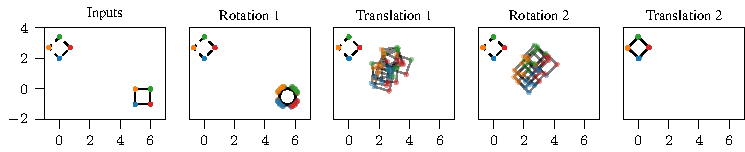
\includegraphics[width=\textwidth]{rotated_squares_example}
    \caption{
        \label{fig:composition:rotated_squares_example}
        Compositional model (toy example): the transformation of the solid rectangle onto the dashed one is decomposed as $T_2 \circ R_2 \circ T_1 \circ R_1$ where $R_i$ and $T_i$ are rotations and translations.
        Different sampled realizations of these transformations are overlaid, showing the \emph{compositional uncertainty}.
        Approximating $R_i$ and $T_i$ as independent transformations does not allow us to capture such uncertainty, collapsing to a single realisation of the composition.
    }
\end{figure}
\begin{figure}[t]
    \centering
    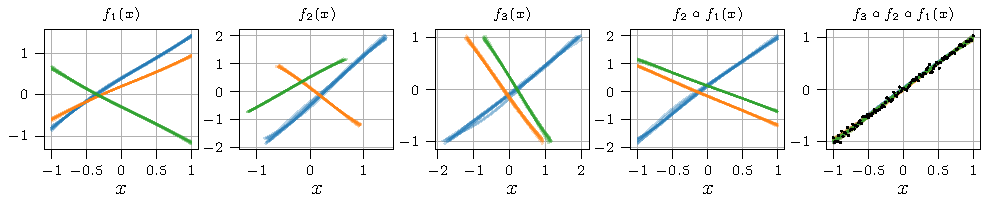
\includegraphics[width=\textwidth]{factorized_dgp_identity}
    \caption{
        \label{fig:composition:identity_factorised}
        Example fits of a three-layer DGP with factorized inducing points to a data set shown in the rightmost panel (black dots).
        Different panels show the computations performed by each of the three layers and their compositions.
        Different colours correspond to three models fitted to the same data with different random initializations.
        For each initialization, ten samples (of the same colour) from the fitted model are shown on top of each other.
    }
\end{figure}
The experiments in~\cref{toc:data_association} showed that data association problem generally do not have a unique solution.
Besides exchanging modes entirely, the spatial priors in the Bayesian association model allow for qualitatively different explanations of the data, all of which conform similarly well to the prior and result in similar marginal likelihoods.
Since all explanations are plausible, a full Bayesian posterior should contain all possible associations and generating processes.
Marginalizing all plausible model realizations would take all possible solutions of the assignment problem into account.
This full posterior is highly complex however, containing strong dependencies between the different components of the hierarchical model.
In this section, we describe why the variational inference schemes from~\cref{toc:dgp} based on strong independence assumptions can only represent posteriors of limited complexity.
For additional details and detailed experiments, we refer to the associated publication~\parencite{ustyuzhaninov_compositional_2020}.

\Cref{fig:composition:rotated_squares_example} illustrates this complexity in a toy example of mapping a square to another square in the two-dimensional euclidean plane.
We formulate an overparameterized hierarchical model by representing the required affine transformation as the chain $T_2 \circ R_2 \circ T_1 \circ R_1$, with the $T_i$ representing translations and the $R_i$ representing rotations.
The task can be solved by an arbitrary choice of $T_1$ and $R_1$ and corresponding choices $T_2 = T_\ast \circ T_1\inv$ and $R_2 = R_\ast \circ R_1\inv$ with $T_\ast \circ R_\ast$ representing the unique correct transformation from one square to the other.
This example illustrates that the notion of a correct hierarchical posterior is problematic:
A posterior model might assign non-zero probability to all possible choices of the first rotation and transformation and a delta-distribution for the correct corresponding choice of the second rotation and transformation.
Alternatively, a posterior might choose $T_1$ and $R_1$ to be identity mappings and $T_2 = T_\ast$ and $R_2 = R_\ast$.
While the first posterior might be considered a more correct Bayesian posterior correctly representing unidentifiable parts of the learning problem, the second posterior is arguably simpler and represents the uniqueness of the correct solution better.
Since both solutions explain the data equally well, this question might not be a problem in practice if the goal is to design a model that provides high marginal likelihood of the data.
In situations where reasoning about internal structure of a hierarchical model such as in~\cref{toc:alignment} or generalization behavior such as in~\cref{toc:interpretable_rl} come into focus, informative posterior distributions over hierarchical generative processes can allow us to build more interpretable models and represent multiple qualitatively different solutions.

The original variational inference scheme for deep GP models by \textcite{damianou_deep_2013} is prohibitively expensive for large data sets.
To overcome this limitation, the inference schemes presented in~\cref{toc:dgp} make strong independence assumptions between different components in a deep GP.
While these assumptions allow training deep GPs with large amounts of data, assuming independence between the different $f_i$ in a compositional prior $f_L \circ \dots \circ f_1$ significantly limits the expressiveness of model posteriors, since every realization of the composition must map the same input to the same output.
\Cref{fig:composition:identity_factorised} shows a comosition of three linear functions, each of which with either positive or negative slope which together should represent the identity function.
The choice of slope for $f_3$ depends on the choice of $f_1$ and $f_2$.
The colors represent different results of training.
Since the $f_i$ are assumed to be independent, the only way to ensure that every realization of the posterior fits the data is to collapse to deterministic functions.
This intuition also holds for general deep GPs, where qualitatively different choices in mappings closer to the input cannot lead to corresponding choices closer to the output.

The model discussed in~\cref{toc:alignment} yields expressive and interpretable uncertainties by formulating a detailled and informed prior paired with a learning problem with inherently high uncertainties due to noise.
Relaxing these requirements to less constrained models requires advances in inference schemes that can represent more expressive posteriors.
Recent work extends the variational approximations with dependencies between layers~\parencite{ustyuzhaninov_compositional_2020} or proposes inference based on stochastic gradient Hamilton Monte Carlo~\parencite{havasi_inference_2018}.
While in their current state, such inference schemes are computationally expensive, they present promising directions of research.

\section{Surrogate models for Bayesian optimization}
\label{toc:discussion:bo}
Above we have argued that in hierarchical models, a high marginal likelihood may not be sufficient to identify desirable solution because the marginal likelihood does not take internal structure into account.
In this section, we consider a complementary situation, where a model is embedded in a hierarchy.
We consider Bayesian optimization (BO)~\parencite{snoek_practical_2012}, where an (often non-hierarchical) regression model is used to solve an optimization problem based on limited observations of the objective function.
We make an argument why surrogate models with suboptimal marginal likelihood can be the model of choice for solving the downstream task.
For additional details about the model and detailed experiments, we refer to the associated publication~\parencite{bodin_modulating_2020}.

BO is a method for finding the optimum of functions that are unknown and expensive to evaluate.
Let $f : \Xc \to \Rb$ be an unknown, noise-free objective function defined on a bounded subset $\Xc \subset \Rb^k$ for some $k \in \Nb$.
The goal of BO is to solve the global optimization problem of finding
\begin{align}
    \mat{x}_\ast \in \argmin_{\mat{x} \in \Xc} f(\mat{x}).
\end{align}
By fitting a surrogate model to samples of an unknown objective, the BO procedure iteratively picks new samples for evaluation that are believed to be the most informative about where the optimum is located.
In real world problems, the objective function is often not a well-behaved function and a suitable model is difficult to specify.
A misspecified model can be especially problematic in sequential decision making tasks such as BO, where the model is not only used to locate the optimum based on the collected data but also to decide where to collect data for future decisions.

There are many approaches to avoiding model misspecification in surrogate models for BO based on additional structure.
For example, GP surrogates can be augmented with warpings to model non-stationarity~\parencite{snoek_input_2014}, separate the input space via tree-structures~\parencite{jenatton_bayesian_2017} or optima can be searched via pairwise comparison~\parencite{gonzalez_preferential_2017}.
While carefully chosen extensions can avoid misspecification, inference over more sophisticated surrogates often requires more observations, which is not desirable in the BO setting.
Importantly, the ultimate goal of BO is to locate the optimum, not to model the objective as precisely as possible.
In practice, surrogates with high complexity often perform worse compared to simpler ones even if the former contains the true objective function while the latter does not.

To formalize this observation, we consider the family of objective functions $f$ that can be represented as a composition
\begin{align}
    f(\mat{x}) = g(\mat{x}, \mat{h}), \quad \mat{h}=h(\mat{x}),
\end{align}
where $g$ is a well-behaved function that can be nicely modeled by a BO surrogate and the nuisance function $h(\mat{x})$ encodes the structures the surrogate model struggles to capture.
Instead of building a complex surrogate model with minimal model misspecification, we propose to explicitly trade off accuracy in modeling the objective with efficiency of capturing informative structures from small amounts of data.
For example, local oscillations and discontinuities are less important to capture in a BO setting than describing global trends.

\begin{figure}[t]
    \centering
    \raisebox{-0.5\height}{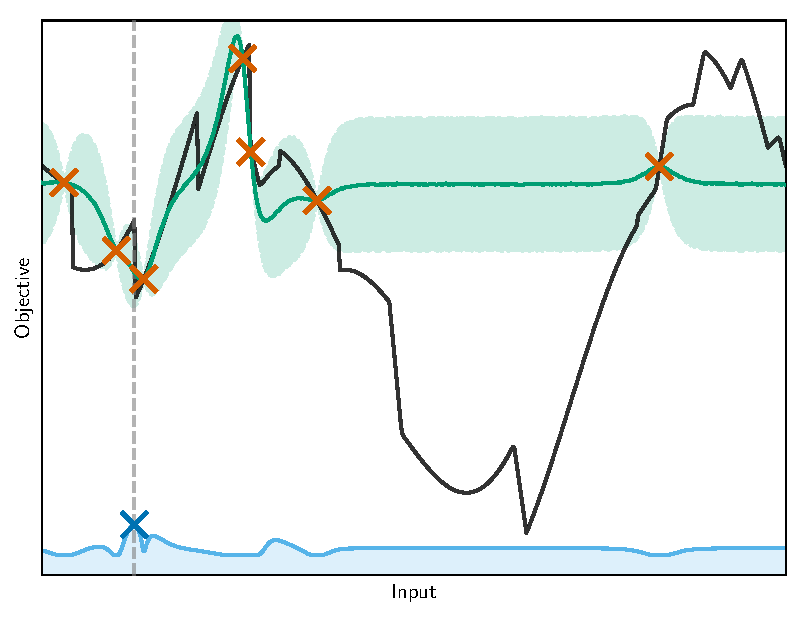
\includegraphics[trim=15 15 0 0, clip, width=0.25\textwidth]{robust_bo_erik/illustrative_figure/gp.pdf}}
    \raisebox{-0.5\height}{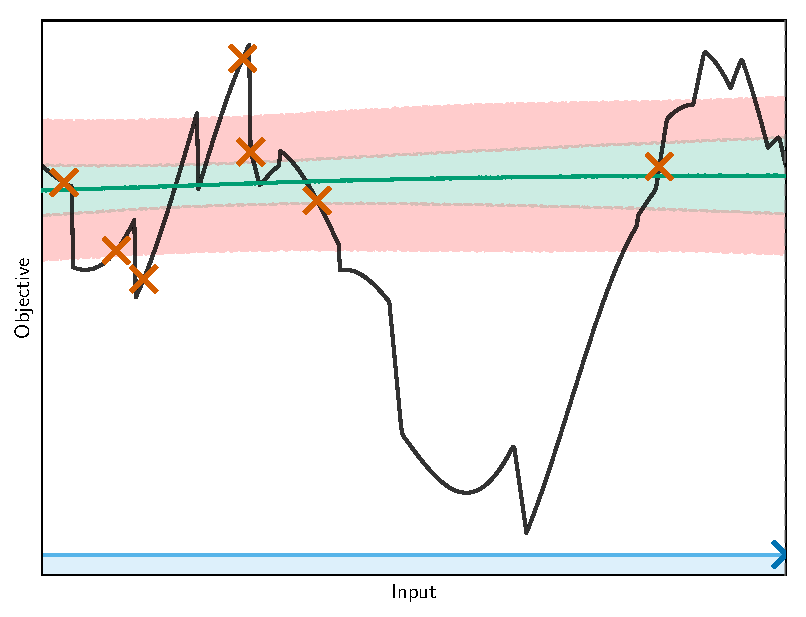
\includegraphics[trim=15 15 0 0, clip, width=0.25\textwidth]{robust_bo_erik/illustrative_figure/homo_gp.pdf}}
    \raisebox{-0.5\height}{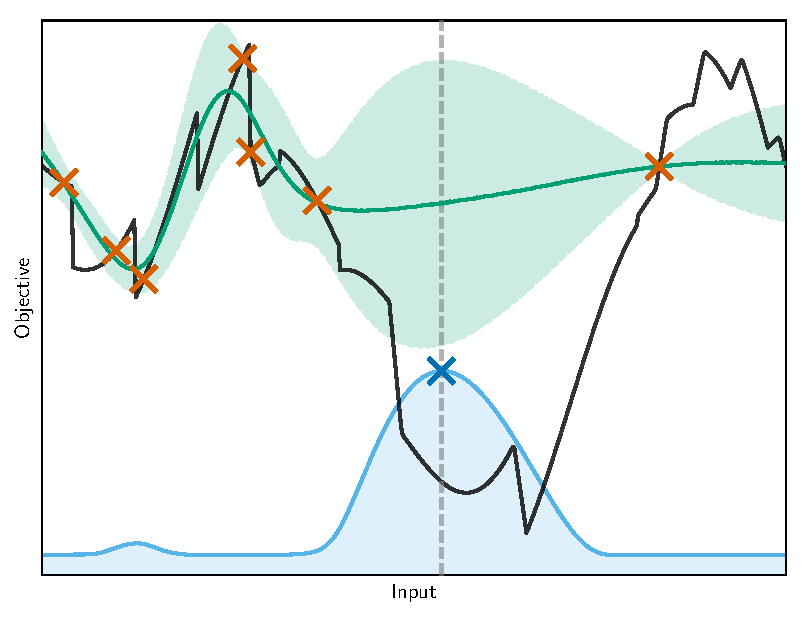
\includegraphics[trim=15 15 0 0, clip, width=0.25\textwidth]{robust_bo_erik/illustrative_figure/modulating_lgp.pdf}}
    \raisebox{-0.45\height}{{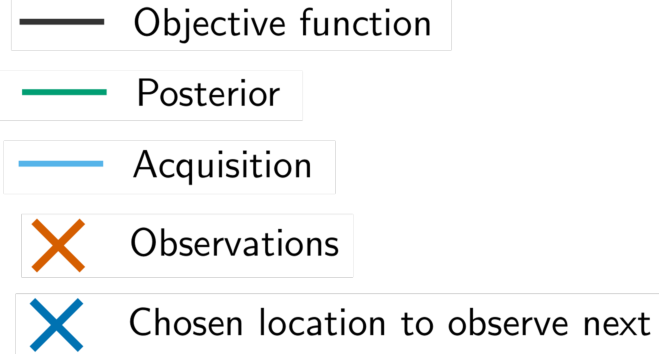
\includegraphics[width=0.20\textwidth]{robust_bo_erik/illustrative_figure/legend_compact.pdf}}}
    \caption{
        \label{fig:bo:posterior}
        As a result, the acquisition function can utilize a confidently discovered global trend to increase the efficiency of the search.
    }
\end{figure}
Assuming additive structure $f(\mat{x}) = g(\mat{x}) + h(\mat{x})$ and choosing the nuisance function to be input-independent noise $h(\mat{x}) \sim \Gaussian{\mat{0}, \sigma^2 \Eye}$ recovers GP regression with a Gaussian likelihood.
For richer structure, we place a GP prior on $g(\mat{x}, \mat{h})$ and infer independent latent variables $\mat{h} \sim \Gaussian{\mat{0}, \sigma^2 \Eye}$ for all observations $\mat{x}$, giving rise to a Latent Gaussian process (LGP)~\parencite{pfingsten_nonstationary_2006,wang_gaussian_2012,yousefi_unsupervised_2016,bodin_latent_2017}.
Intuitively, increasing the absolute value of $\mat{h}$ is penalized by the prior but allows the surrogate to not interpolate an observation exactly and to ignore local structure.
Similar to using noiseless predictions with Gaussian likelihoods, we ignore the nuisance parameters $\mat{h}$ in the search for the optimum and focus on the global trends captured by $g(\mat{x}, \mat{0})$.

\Cref{fig:bo:posterior} compares three surrogates on a function with challenging local structure.
A standard noiseless GP interpolates all observations exactly and must capture all local variations.
Since this surrogate quickly reverts to the prior between observations, it cannot capture global trends and therefore is not very helpful in solving the global optimization problem.
The LGP-based surrogate ignore local structure and does not interpolate observations exactly, which leads to a reduced marginal likelihood.
However, the model uncovers a global trend, which allows the BO-scheme to identify the correct area of interest.

The experiments in~\parencite{bodin_modulating_2020} give empirical evidence that this intuition holds for many BO tasks.
The approach performs especially well in high-dimensional problems, where global trends tend to matter more in low-data regimes due to the curse of dimensionality.
The idea that a surrogate in BO need not model the objective perfectly but yield informative insights for the optimization task was not formally included in the model formulation in this section.
Instead, we considered a class of surrogates that implicitly have this property.
In the next section, we go one step further and include the task of policy search in the inference problem of reinforcement learning explicitly.


\section{Bayesian Reinforcement Learning}
\label{toc:discussion:mountaincar}
\begin{table}[t]
    \caption[Statistical learning methodology in reinforcement learning]{
        \label{tab:mountaincar:quantities_of_interest}
        Mapping of the statistical learning methodology to the reinforcement learning problem.
    }
    \centering
    \includestandalonewithpath{figures/quantities_of_interest_statistical_learning}\\[\figureskip]
    \newcolumntype{Y}{>{\centering\arraybackslash}X}
    \begin{tabularx}{.9\textwidth}{cYY}
        \toprule
                                  & Statistical learning   & Reinforcement learning \\
        \midrule
        $\Prob*{\mat{z}}$         & Latent distribution    & True system-dynamics   \\
        $\Sc$                     & Observations           & Batch or online data   \\
        $\Fc$                     & Functional of interest & Optimal value          \\
        \midrule
        $F : \Probs{\Zc} \to \Fc$ & Functional operator    & Bellman principle      \\
        $S : \Probs{\Zc} \to \Sc$ & Sampling operator      & Exploration            \\
        $A : \Sc \to \Fc$         & Learning algorithm     & Policy search          \\
        \bottomrule
    \end{tabularx}
\end{table}
In statistical learning, the goal is to learn about an unknown latent probability distribution via a limited number of observations.
The goal of learning is to recover some projection or functional of interest of the latent distribution.
In this thesis, we have mostly focused on the regression setting, where the goal is to learn the marginal $\Prob*{\mat{y} \given \mat{x}}$ of a data distribution $\Prob*{\mat{x}, \mat{y}}$.
We have formulated hierarchical models to incorporate prior knowledge about the generative process that informs the data distribution.
We have argued that a high marginal likelihood may not be enough to identify a desirable hierarchical model that, besides reproducing data, also captures the true generative process well.

In~\cref{toc:interpretable_rl}, we saw that well specified models solve decision problems in reinforcement learning significantly better than misspecified problems, even if they represent training data equally well.
In this section, we formalize this insight and formulate the policy search problem in reinforcement learning via a generative process.
This allows us to include the requirement for good performance in the inference problem and reason about it in a Bayesian manner.
In~\cref{tab:mountaincar:quantities_of_interest}, we show how policy search in reinforcement learning problem can be formulated as a statistical learning problem.
Based on latent true system dynamics, our goal is to identify the optimal value function and thus an optimal policy based on a limited number of interactions with the system.
The optimal value is defined via the Bellman principle~\parencite{sutton_reinforcement_2018}, which is hard to apply directly in general.
Instead, we observe batch or online data and apply an algorithm for policy search.

\begin{figure}[t]
    \centering
    \includestandalone{graphical_model_rl_deep_gp}
    \caption{
        \label{fig:mountaincar:graphical_model}
        Deep GP RL graphical model.
    }
\end{figure}
Our goal is to formulate policy search in reinforcement learning as an inference problem in a hierarchical model.
We start by interpreting the definition of the $T$-step value function
\begin{align}
    J^\pi(\mat{s}_0) = \Moment*{\E}{\sum_{t=1}^T \gamma^t r(\mat{s}_t) \given f, \pi}
\end{align}
as a generative process with the associated graphical model~\cref{fig:mountaincar:graphical_model}.
Starting with the initial state $\mat{s}_0$, trajectories are generated using the transition dynamics $f$ and policy $\pi$.
If both the transition dynamics and policy are represented as GPs, the graphical model of a trajectory is a recurrent deep Gaussian process.
The states are mapped to rewards using the known reward function $r$ and added to produce the value $J^\pi$, thereby defining a likelihood function.
Instead of considering the value of any arbitrary policy $\pi$, we now reason about the uniquely defined optimal value $J_\ast$.
Since the optimal value can be parameterized by an optimal policy $\pi_\ast$, it can be represented in our hierarchical model.
Our goal is to formulate an equivalent to the marginal likelihood of the optimal value function and derive an inference scheme.

There are two distinct sources of uncertainty in this model.
First, knowledge of the dynamical system can be imperfect or the system can be stochastic in nature.
Both effects make trajectories non-deterministic, even if the initial state and policy are fixed.
This kind of uncertainty is reflected in the expected value of the original value definition and we retain these uncertainties.
Second, we do not maintain a candidate policy we want to optimize and approximate the optimal value instead.
Since our knowledge about the optimal policy is imperfect, so is our knowledge about the optimal value.
Both uncertainties are captured in the distribution $\Prob*{J_\ast \given \mat{s}_0}$.

To formulate an equivalent of the marginal likelihood, we can bound the optimal value function.
We assume without loss of generality that the reward function is bounded and that $\max_{\mat{s}} r(\mat{s}) = 0$.
Then we have that
\begin{align}
    \label{eq:mountaincar:inequality_chain}
    \forall \mat{s} \forall \mat{\pi} : J^\pi(\mat{s}) \leq J^{\pi^\ast}(\mat{s}) \leq J^\text{max} \coloneqq \sum_{t=0}^T \gamma^t \cdot 0 = 0,
\end{align}
that is, any arbitrary policy will achieve a value less than or equal to the optimal policy and the optimal value can never be higher than the sum of maximum achievable rewards.
Given by the structure discussed above we have
The graphical model implies the marginal likelihood
\begin{align}
    \label{eq:mountaincar:true_likelihood}
    \Prob{\mat{J}^{\pi^\ast} \given \mat{s}_0}
     & = \int
    \underbrace{\Prob{\mat{J}^{\pi^\ast} \given \mat{J}}}_{\text{Likelihood}}
    \underbrace{\Prob{\mat{J} \given \mat{\pi}^\ast, \mat{s}_0, \mat{f}}}_{\text{Trajectory}}
    \underbrace{\Prob{\mat{\pi}^\ast, \mat{f}}}_{\text{System}}
    \diff \mat{J} \diff \mat{\pi}^\ast \diff \mat{f} \diff \mat{s}_0,
    \\
    \label{eq:mountaincar:max_likelihood}
     & \geq \int
    \Prob{\mat{J}^{\text{max}} \given \mat{J}}
    \Prob{\mat{J} \given \mat{\pi}^\ast, \mat{s}_0, \mat{f}}
    \Prob{\mat{\pi}^\ast, \mat{f}}
    \diff \mat{J} \diff \mat{\pi}^\ast \diff \mat{f} \diff \mat{s}_0,
\end{align}
where the inequality is implied by \cref{eq:mountaincar:inequality_chain} if the likelihood is monotonically decreasing with distance.
Both the trajectory and system terms can easily be interpreted, as they represent the recurrent structure and function approximators respectively.
It is not clear, however, how to interpret the likelihood term.
Given the value estimate $\mat{J}$, this term encapsulates an estimation of closeness to the optimal value and must encode that the optimal value is the highest possible value.

\begin{figure}[t]
    \centering
    \includestandalone{mountaincar_system}
    \caption{
        \label{fig:mountaincar:system}
        Mountaincar system
    }
\end{figure}
We now assume variational distributions $\Variat{\mat{f}}$ and $\Variat{\mat{\pi}^\ast}$ introduced by the sparse GP formulations in~\cref{toc:dgp}.
Analogously to the derivation of the DSVI-bound in~\cref{eq:dsvi:full_bound} we get
\begin{align}
    \begin{split}
        \label{eq:mountaincar:variational_bound}
        \log \Prob{\mat{J}^{\pi^\ast} \given \mat{s}_0}
        & \geq \log \Prob{\mat{J}^{\text{max}} \given \mat{s}_0}        \\
        & = \log \int
        \Prob{\mat{J}^{\text{max}} \given \mat{J}}
        \Prob{\mat{J} \given \mat{\pi}^\ast, \mat{s}_0, \mat{f}}
        \Prob{\mat{\pi}^\ast, \mat{f}}
        \diff \mat{J} \diff \mat{\pi}^\ast \diff \mat{f} \diff \mat{s}_0 \\
        & \geq
        \Moment*{\E_{\Variat{\mat{s}_0, \dots, \mat{s}_T}}}{
        \log \int
        \Prob{\mat{J}^{\text{max}} \given \mat{J}}
        \underbrace{\Prob{\mat{J} \given \mat{s}_0, \dots, \mat{s}_T}}_{\text{Deterministic}}
        \diff \mat{J}
        }
        - T \cdot \text{klterm}
        \\
        & =
        \Moment*{\E_{\Variat{\mat{J}}}}{\log \Prob{\mat{J}^{\text{max}} \given \mat{J}}}
        - T \cdot \text{klterm},
    \end{split}
\end{align}
with $\text{klterm} = \KL{\Variat{\mat{\pi}^\ast}}{\Prob{\mat{\pi}^\ast}} + \KL{\Variat{\mat{f}}}{\Prob{\mat{f}}}$ multiplied by $T$ due to the recurrent structure.
The distribution $\Variat{\mat{J}}$ can easily be sampled from $\Variat{\mat{s}_0, \dots, \mat{s}_T}$ using the definition of the value function.
A sample from $\Variat{\mat{s}_0, \dots, \mat{s}_T}$ can be drawn via the usual ancestral sampling scheme employed by DSVI.
Assuming that the sufficient statistics assumption holds for both $\mat{\pi}^\ast$ and $\mat{f}$, the optimal policy is still maximizes variational lower bound if $\Prob*{\mat{J}^{\text{max}} \given \mat{J}}$ is monotonous.
We choose an exponential likelihood, that is
\begin{align}
    \begin{split}
        \Prob{\mat{J}^\text{max} \given \mat{J}}
        &\coloneqq \lambda \Fun{\exp}{-\lambda (\mat{J}^\text{max} - \mat{J})} \\
        &= \lambda \Fun{\exp}{\lambda \mat{J}},
    \end{split}
\end{align}
since $\mat{J}^\text{max} = 0$.
With $\lambda = 1$, the bound in \cref{eq:mountaincar:variational_bound} reduces to
\begin{align}
    \begin{split}
        \MoveEqLeft\Moment*{\E_{\Variat{\mat{J}}}}{\log \Prob{\mat{J}^{\text{max}} \given \mat{J}}} - T \cdot \text{klterm}
        \\
        &= \Moment*{\E_{\Variat{\mat{J}}}}{\log \Fun{\exp}{\mat{J}}} - T \cdot \text{klterm}
        \\
        &= \Moment*{\E_{\Variat{\mat{J}}}}{\mat{J}} - T \cdot \KL{\Variat{\mat{\pi}^\ast}}{\Prob{\mat{\pi}^\ast}} + \text{const}.
    \end{split}
\end{align}
This bound is similar to a standard policy iteration scheme but is also subject to the prior on $\mat{\pi}^\ast$.

\begin{figure}[tp]
    \centering
    \includestandalone{mountaincar_policy_01}
    \includestandalone{mountaincar_policy_10}
    \includestandalone{mountaincar_policy_25}
    \caption{
        \label{fig:mountaincar:policy}
        Mountaincar policies after different iteration counts.
    }
\end{figure}
As an example, we consider the mountain car system~\parencite{moore_efficient_1990,sutton_reinforcement_2018}.
\Cref{fig:mountaincar:system} visualizes the task of driving an underpowered car up a mountain.
The car's engine is not strong enough to overcome the slope and a successful agent must first drive away from the goal on the right to build momentum.
The current state of the benchmark is described by the one-dimensional position and velocity of the car and the agent can accelerate the car in either direction.

We train a dynamics model with random observations of the system and maximize the variational bound in~\cref{eq:mountaincar:variational_bound} to find an optimal policy to solve the benchmark problem.
\Cref{fig:mountaincar:policy} shows how the Bayesian belief about the optimal policy evolves during optimization of the bound.
Starting off with an uninformed policy for which all actions are plausible in all states, the approximation of the optimal value is very uncertain and uninformed.
During training, the areas iun the input space which are relevant for solving the task emerge and a successful policy is found that oscillates in the valley to build momentum and overcome the mountain.
The inference scheme also uncovers areas in the input space where uncertainty about the optimal policy is never reduced.
Since this policy representation is used to parameterize the optimal value, these states are not relevant for a good approximation.
In other words, these states are either never reached or all actions lead to success.

Formulating policy search as an inference problem over the optimal value allows us to automatically uncover which parts of a system are relevant to solving a task.
Similar to a surrogate in BO not needing to fully represent complicated structure away from the optimum, both a dynamics model and policy representation need not understand a system fully to solve a reinforcement learning task.
Separating a system in relevant and irrelevant parts to steer exploration or policy search are promising directions of research.


\section{Future work}
\label{toc:discussion:future_work}
Taking the step to applying machine learning in the physical world is one of the most important challenges for machine learning today.
ML-systems that operate in safety-critical areas, interact with people, or carry responsibility must be robust, trustworthy, and assessable.
This thesis explored how structured Gaussian process models can be used to formalize abstract knowledge about hierarchical systems and gain new insights from data.
Future research will allow us to generalize these results and explore the following questions:
\begin{itemize}
    \item How do we formulate data-efficient models together with domain experts?
    \item How do we ensure models can be trusted to take responsibility?
    \item How do we implement models to yield robust results?
\end{itemize}

Machine learning models can be effective tools for communication with experts if they allow extensive inspection to achieve interpretability.
Formulating principled generative models based on expert understanding allows us to reproduce abstract expectations and combining such models with data allows us to gain new insights about the badly understood components of a system.
In \cref{toc:discussion:bo,toc:discussion:mountaincar} we discussed approaches to including downstream tasks in modeling problems.
Bayesian learning in piplines of tasks is an active area of study in probabilistic numerics~\parencite{cockayne_bayesian_2019}, where multiple numerical algorithms are applied in succession.
It is an interesting research question how these ideas can be implemented in more general problem settings where priors and expectations are less well defined.

In Bayesian inference, a model is typically evaluated with respect to subjective prior belief and the likelihood of observations which are typically assumed to be independent.
Hierarchical models are often formulated with components that have clear responsibilities to allow experts to independently reason about the prior assumptions of different parts of a model.
However, we have seen in~\cref{toc:discussion:composition} that once we include compositions of general function approximators in a generative model, strong dependency structures emerge and reasoning about priors is difficult~\parencite{duvenaud_avoiding_2014}.
Future work will explore how to constrain hierarchical models beyond componentwise structural assumptions.
Hierarchical models such as the alignment model in~\cref{toc:alignment} can show rich and expert-interpretable structure in the shape of samples drawn from generative models.
One interesting direction of research is to explore how to formalize expectations about such samples as a new way to place constraints on the internal structure of hierarchical models.

Interpretable models and principled uncertainty propagation often require costly computations.
To implement models in practice, we need to rely on more efficient approximations which can limit the range of representable solutions.
As we have seen in~\cref{toc:discussion:composition}, the current approaches to inference in deep Gaussian process models cannot represent complex hierarchical posteriors well and more expressive alternatives tend to be computationally expensive.
The search for efficient and expressive inference schemes for Gaussian processes is an active area of research~\parencite{salimbeni_orthogonally_2018,shi_sparse_2020,wilson_efficiently_2020} and a natural future direction of research is to ask how such schemes can be extended to hierarchical models.
Another interesting question is how to combine the advantages of principled generative models with computationally efficient alternatives.
Large parametric models such as Bayesian neural networks (BNN) allow large-scale inference and fast predictions at the cost of badly understood prior assumptions.
Recent work~\parencite{sun_functional_2019} explored how to formulate Gaussian process priors for BNN models.
It would be interesting to extend these ideas to more informative priors.
